\begin{itemize}

\item Các mẫu chiến lược phân tích nghiệp vụ kinh doanh sau đó đưa ra việc phân chia các thành phần và hiểu mối quan hệ của các thành phần đó.

\item Các mẫu chiến lược là giai đoạn xây dựng sự hiểu biết chung về miền giữa chuyên gia ngành và nhóm phân tích hệ thống.

\item Các mẫu chiến lược giúp xác định các thành phần quan trọng của hệ thống, đảm bảo kiến trúc phần mềm phản ánh đúng các yêu cầu kinh doanh.

$\Rightarrow$ Các mẫu chiến lược xác định mục tiêu tạo ra hệ thống có thể mở rộng, phát triển linh hoạt theo nhu cầu kinh doanh.

bao gồm:

\begin{itemize}

\item Muc1 %!nghia

\item Muc2 %!nghia

\item Muc1 %!nghia

\item Muc2 %!nghia

\item Muc1 %!nghia

\item Muc2 %!nghia

\item Muc1 %!nghia

\item Muc2 %!nghia

\end{itemize}

% nội dung trang lớn lên để hết giấy

\end{itemize}

\begin{figure}[H]

\centering

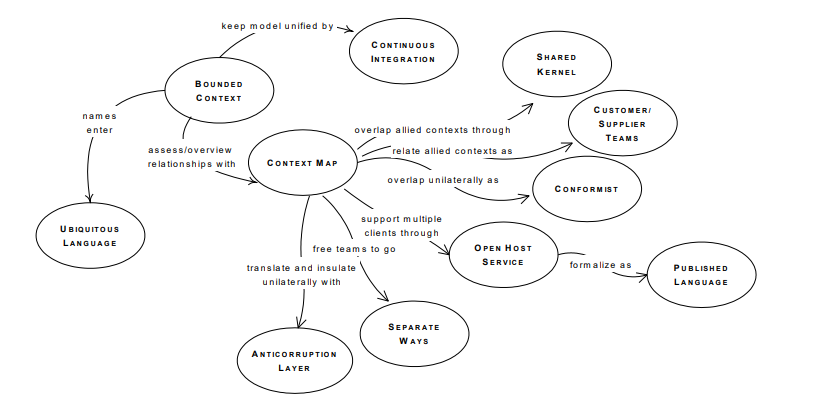
\includegraphics[scale = 0.9]{pictures/cac_mau_chien_luoc/temp.png}

\caption{Sơ đồ về các thành phần trong mô hình chiến lược}

\end{figure}

%!<! - - $ Vẽ lại sau: - - >

%!<! - - $ Vẽ lại sau: - - >

%!<! - - $ Vẽ lại sau: - - >

%!<! - - $ Vẽ lại sau: - - >

%!<! - - $ Vẽ lại sau: - - >

%!<! - - $ Vẽ lại sau: - - >

%!<! - - $ Vẽ lại sau: - - >

%!<! - - $ Vẽ lại sau: - - >

%!<! - - $ Vẽ lại sau: - - >

%!<! - - $ Vẽ lại sau: - - >

